\documentclass{beamer}
\usetheme{Madrid}
\usepackage{xeCJK}
\usepackage{listings}
\usepackage{xcolor}
\usepackage{booktabs}
\usepackage{amsmath}
\usepackage{tikz}
\usetikzlibrary{arrows.meta,positioning}

\definecolor{codegreen}{rgb}{0,0.6,0}
\definecolor{codegray}{rgb}{0.5,0.5,0.5}
\definecolor{codepurple}{rgb}{0.58,0,0.82}
\definecolor{backcolour}{rgb}{0.95,0.95,0.92}
\lstdefinestyle{mystyle}{
    language=C++,
    basicstyle=\small\ttfamily,
    keywordstyle=\color{blue},
    commentstyle=\color{codegreen},
    breaklines=true,
    showstringspaces=false,
}
\lstset{style=mystyle}

\title{面向大模型化学回答的\\可编译分子标记语言与渲染系统}
\author{课程项目汇报}
\institute{Compiler Project}
\date{\today}

\begin{document}

\begin{frame}
    \titlepage
\end{frame}

\begin{frame}{项目动机}
    \begin{itemize}
        \item 化学结构表达天然具有“图”的语义：原子是节点，化学键是边。
        \item 但面向用户书写时，直接写图结构不方便，也不利于错误检查。
        \item 本项目设计一个小型 DSL，用线性文本描述片段组合。
        \item 编译器负责从源语言恢复结构图，并进一步生成分子键线式。
    \end{itemize}

    \vspace{0.5em}
    \begin{block}{核心想法}
        把“分子绘制”建模成一次编译：
        \[
            \text{source program} \rightarrow \text{AST} \rightarrow \text{IR graph} \rightarrow \text{SVG}
        \]
    \end{block}
\end{frame}

\begin{frame}[fragile]{源语言例子}
    一个输入程序：
    \begin{lstlisting}
(0)Ac,1-Cl,(0);
    \end{lstlisting}

    直观含义：
    \begin{itemize}
        \item \texttt{Ac} 是一个关键词片段，表示酰基。
        \item \texttt{1-Cl} 表示在片段的 1 号接口连接氯。
        \item \texttt{(0)} 表示当前连接点或默认端口。
        \item 分号表示一个完整表达式结束。
    \end{itemize}

    \vspace{0.4em}
    编译器不直接把字符串画出来，而是先构造 AST，再翻译成 IR 连接图。
\end{frame}

\begin{frame}{编译管线}
    \centering
    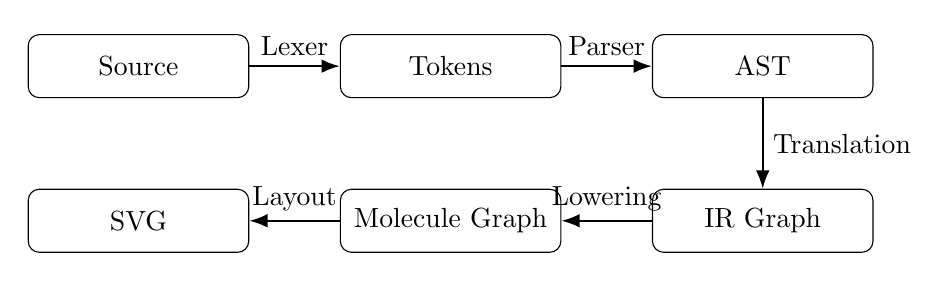
\begin{tikzpicture}[
        node distance=1.15cm,
        box/.style={draw, rounded corners, minimum width=2.8cm, minimum height=0.8cm, align=center},
        arrow/.style={-{Latex}, thick}
    ]
        \node[box] (src) {Source};
        \node[box, right=of src] (tok) {Tokens};
        \node[box, right=of tok] (ast) {AST};
        \node[box, below=of ast] (ir) {IR Graph};
        \node[box, left=of ir] (mol) {Molecule Graph};
        \node[box, left=of mol] (svg) {SVG};

        \draw[arrow] (src) -- node[above]{Lexer} (tok);
        \draw[arrow] (tok) -- node[above]{Parser} (ast);
        \draw[arrow] (ast) -- node[right]{Translation} (ir);
        \draw[arrow] (ir) -- node[above]{Lowering} (mol);
        \draw[arrow] (mol) -- node[above]{Layout} (svg);
    \end{tikzpicture}

    \vspace{0.7em}
    \begin{itemize}
        \item 前端是递归下降 parser。
        \item 中端是 AST 到 IR 的语义翻译。
        \item 后端把 IR graph 交给绘图模块生成 SVG。
    \end{itemize}
\end{frame}

\begin{frame}[fragile]{词法设计}
    源语言中的 token 类型比较少：
    \begin{table}
        \centering
        \begin{tabular}{lll}
            \toprule
            Token & 例子 & 含义 \\
            \midrule
            \texttt{Keyword} & \texttt{Ac}, \texttt{Ph}, \texttt{Cl} & 化学片段名 \\
            \texttt{Number} & \texttt{0}, \texttt{1} & 连接端口编号 \\
            \texttt{Bond} & \texttt{-}, \texttt{=} & 单键或双键 \\
            \texttt{Paren} & \texttt{(}, \texttt{)} & 端口标记 \\
            \texttt{Comma} & \texttt{,} & 同一表达式中的连接项分隔 \\
            \texttt{Semicolon} & \texttt{;} & 一个分子表达式结束 \\
            \bottomrule
        \end{tabular}
    \end{table}

    \begin{lstlisting}
(0)Ac,1-Cl,(0);
    \end{lstlisting}
    词法分析只识别表面符号，不判断 \texttt{Ac} 是否真的存在。
\end{frame}

\begin{frame}[fragile]{语法设计}
    简化后的文法可以写成：
    \begin{lstlisting}
Program   -> ExprList
ExprList  -> Expr ';' ExprList | epsilon
Expr      -> Atom ItemList
ItemList  -> ',' Item ItemList | epsilon
Item      -> Port Bond Atom
           | Port
Atom      -> Port Keyword
           | Keyword
Port      -> '(' Number ')'
           | Number
Bond      -> '-' | '='
Keyword   -> identifier
    \end{lstlisting}

    \vspace{0.3em}
    \begin{itemize}
        \item Parser 根据 token 串构造 AST。
        \item 语法只描述“能不能组成句子”，不负责判断端口是否能连接。
        \item 端口、端基、片段拼接是否合法放到语义翻译阶段检查。
    \end{itemize}
\end{frame}

\begin{frame}{AST 结构}
    \centering
    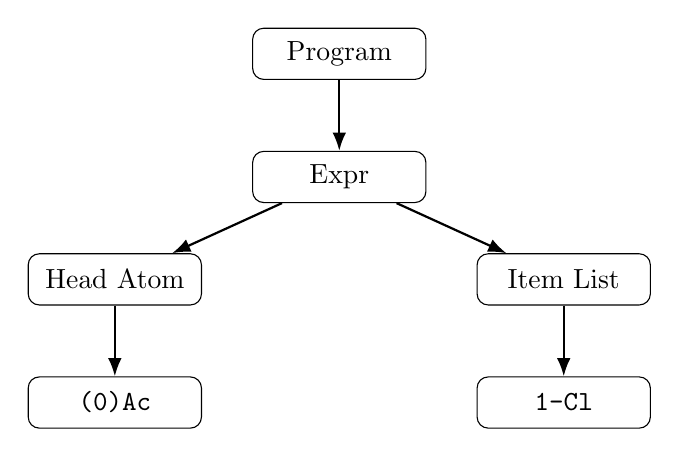
\begin{tikzpicture}[
        node distance=0.9cm,
        box/.style={draw, rounded corners, minimum width=2.2cm, minimum height=0.65cm, align=center},
        arrow/.style={-{Latex}, thick}
    ]
        \node[box] (program) {Program};
        \node[box, below=of program] (expr) {Expr};
        \node[box, below left=of expr] (head) {Head Atom};
        \node[box, below right=of expr] (items) {Item List};
        \node[box, below=of head] (ac) {\texttt{(0)Ac}};
        \node[box, below=of items] (cl) {\texttt{1-Cl}};

        \draw[arrow] (program) -- (expr);
        \draw[arrow] (expr) -- (head);
        \draw[arrow] (expr) -- (items);
        \draw[arrow] (head) -- (ac);
        \draw[arrow] (items) -- (cl);
    \end{tikzpicture}

    \vspace{0.5em}
    AST 保留源语言的层次结构；IR 不再关心逗号、括号等语法细节，只关心图连接。
\end{frame}

\begin{frame}{属性文法 / SDT 思路}
    对每个 AST 节点综合一个属性：
    \[
        node.frag = \langle V, E, entry, exit \rangle
    \]

    \begin{itemize}
        \item \(V\)：IR 中的原子节点集合。
        \item \(E\)：IR 中的化学键集合。
        \item \(entry\)：这个片段被外部连接时使用的入口。
        \item \(exit\)：继续向右拼接时使用的出口。
    \end{itemize}

    \vspace{0.5em}
    \begin{block}{端基}
        \(\texttt{exit = None}\) 表示这个片段是端基。
        它可以被接到别的片段上，但不能再继续作为左侧片段向外延伸。
    \end{block}
\end{frame}

\begin{frame}[fragile]{翻译动作示例}
    关键词首先被翻译成基础 fragment：
    \begin{lstlisting}
Keyword("Cl").frag = {
  nodes = { Cl },
  edges = { },
  entry = Cl,
  exit = None
}

Keyword("Ac").frag = {
  nodes = { C, O, C },
  edges = { C=O, C-C },
  entry = C,
  exit = C
}
    \end{lstlisting}

    \vspace{0.5em}
    之后连接规则把两个 fragment 的接口合并，并插入对应键。
\end{frame}

\begin{frame}{语义检查}
    语法正确不代表语义正确。翻译阶段会检查：
    \begin{itemize}
        \item 关键词是否存在于 Keyword 表中。
        \item 连接端口是否存在。
        \item 被连接的 fragment 是否有可用 entry。
        \item 左侧 fragment 是否还有 exit 可以继续拼接。
        \item 端基是否被错误地继续扩展。
    \end{itemize}

    \vspace{0.5em}
    \begin{block}{例子}
        如果整体 \(\texttt{exit = None}\)，但后面仍然出现需要继续拼合的项，
        翻译阶段会报错，而不是生成错误的分子图。
    \end{block}
\end{frame}

\begin{frame}{IR 设计}
    IR 是一个显式连接图：
    \begin{itemize}
        \item \textbf{IrNode}：原子或抽象节点，保存元素类型。
        \item \textbf{IrEdge}：节点之间的化学键，保存键阶。
        \item \textbf{Fragment}：可组合的图片段。
        \item \textbf{Program IR}：多个 fragment 拼接后的整体图。
    \end{itemize}

    \vspace{0.5em}
    \begin{block}{为什么需要 IR}
        AST 适合表达语法结构；IR 适合表达语义结构。
        从 AST 到 IR 的转换，正是本项目的核心编译步骤。
    \end{block}
\end{frame}

\begin{frame}[fragile]{递归下降解析}
    文法规模较小，因此 parser 采用手写递归下降：
    \begin{itemize}
        \item 每个非终结符对应一个解析函数。
        \item 通过当前 token 判断产生式分支。
        \item 解析失败时抛出带位置的语法错误。
        \item 解析成功后返回 AST 节点，而不是立即生成 IR。
    \end{itemize}

    \begin{lstlisting}
parseExpr():
  head = parseAtom()
  items = parseItemList()
  return Expr(head, items)

parseItemList():
  while match(','):
    items.push_back(parseItem())
    \end{lstlisting}

    这样把语法分析和语义翻译分离，便于单独打印 AST 和 IR。
\end{frame}

\begin{frame}{后端与展示}
    \begin{itemize}
        \item IR 被进一步转换为分子连接图。
        \item 后端生成 SVG，用来验证 IR 是否正确。
        \item 浏览器插件只是展示外壳，不是本课程项目的主要编译内容。
    \end{itemize}
\end{frame}

\begin{frame}{当前完成度与后续工作}
    \begin{columns}
        \begin{column}{0.48\textwidth}
            \textbf{已完成}
            \begin{itemize}
                \item 词法与语法分析
                \item 递归下降 Parser
                \item AST 到 IR 翻译
                \item Keyword 独立模块
                \item 端基和端口语义检查
                \item SVG 输出用于验证
            \end{itemize}
        \end{column}
        \begin{column}{0.48\textwidth}
            \textbf{后续方向}
            \begin{itemize}
                \item 扩展关键词片段库
                \item 更完善的错误诊断
                \item 与 SMILES 输出做对比
                \item 建立测试集统计成功率
                \item 改进复杂环系表达能力
            \end{itemize}
        \end{column}
    \end{columns}
\end{frame}

\begin{frame}{总结}
    \begin{itemize}
        \item 本项目把分子结构绘制抽象成一个小型语言的编译问题。
        \item 前端完成 token 化、递归下降解析和 AST 构造。
        \item 中端通过属性/SDT 思路，把 AST 翻译为 IR 连接图。
        \item 语义检查集中处理关键词、端口、端基和 fragment 拼接合法性。
    \end{itemize}

    \vspace{0.8em}
    \centering
    \Large{谢谢！}
\end{frame}

\end{document}
